\documentclass[11pt]{article}

\topmargin = 0mm
\textwidth = 150mm 
\oddsidemargin = 0mm

\usepackage[utf8]{inputenc}
\usepackage[russian]{babel}
\usepackage{graphicx}
\usepackage{caption}
\usepackage{amsmath}
\usepackage{amssymb}
\usepackage{listings}
\usepackage{float}
\usepackage{graphicx}
\usepackage{subfig}
\usepackage{bm}
\usepackage{comment}
\usepackage[ruled]{algorithm2e}
\usepackage{systeme}

\DontPrintSemicolon

\SetKwInput{KwData}{Исходные параметры}
\SetKwInput{KwResult}{Результат}
\SetKwInput{KwIn}{Входные данные}
\SetKwInput{KwOut}{Выходные данные}
\SetAlgorithmName{Алгоритм}{алгоритм}{Список алгоритмов}

\DeclareMathOperator{\diag}{diag}  

\title{Методы оптимизации в машинном обучении \\
Отчет по практическому заданию №2}
\author{Коробов Павел, группа 517}

\begin{document}


\maketitle
\thispagestyle{empty}

\section{Введение.}
В данном задании мы изучим работу метода логарифмических барьеров на примере оптимизации LASSO-регрессии. 

\section{Оптимизация LASSO-регрессии методом логарифмических барьеров.}
Сформулируем задачу LASSO-регрессии. 
Пусть имеется обучающая выборка $\left(\left(a_{i}, b_{i}\right)\right)_{i=1}^{m}$, где $a_{i} \in \mathbb{R}^{n}$ -- вектор признаков $i$-го объекта, а $b_{i} \in \mathbb{R}$ -- его регрессионное значение.
Задача заключается в прогнозировании регрессионного значения $b_{\text {new }}$ для нового объекта, представленного своим вектором признаков $a_{\text {new }}$.
Коэффициенты $x$ модели настраиваются с помощью решения следующей оптимизационной задачи:

$$\frac{1}{2} \sum_{i=1}^{m}\left(\left\langle a_{i}, x\right\rangle-b_{i}\right)^{2}+\lambda \sum_{j=1}^{n}\left|x_{j}\right|= \frac{1}{2}\|A x-b\|^{2}+\lambda\|x\|_{1} \rightarrow \min _{x \in \mathbb{R}^{n}}.$$

Здесь $\lambda > 0$ -- коэффициент регуляризации.

Можно преобразовать данную задачу через надграфик:

$$\min _{x, u \in \mathbb{R}^{n}}\left\{\frac{1}{2}\|A x-b\|^{2}+\lambda\left\langle 1_{n}, u\right\rangle\right\} \quad \text { s.t. } \quad-u \preceq x \preceq u$$

Выпишем для этой задачи воспомогательную функцию для метода барьеров. В качестве барьерной функции возьмем логарифмический барьер $F(x):=-\sum_{i=1}^{m} \ln \left(-g_{i}(x)\right)$.

Множество $Q$ задается следующими $2n$ ограничениями:
	$$g_i^+ = x_i - u_i, \quad g_i^-(x, u) = -x_i - u_i, \quad 1 \leq i \leq n$$

Тогда вспомогательная функция будет выглядеть следующим образом.

$$f_{t}(x, u) = t \left( \frac{1}{2} \|A x-b\|^{2}+\lambda\left\langle 1_{n}, u\right\rangle \right) - \sum_{i=1}^{n} \ln \left(u_i - x_i\right) - \sum_{i=1}^{n} \ln \left(x_i + u_i\right)$$

Минимизируем  квадратичную модель в точке $x_k$:

$$
f \left( \tilde{x}_{k}+d \right) \approx m_{k}(d) = f \left(\tilde{x}_{k}\right)+\nabla f\left(\tilde{x}_{k}\right)^{T} d+\frac{1}{2} d^{\top} B_{k} d \rightarrow \min,$$

где $\tilde{x} = \begin{pmatrix} x \\ u \end{pmatrix}$, $d = \begin{pmatrix} d^x \\ d^u \end{pmatrix}$.

В случае метода Ньютона $B_k = \nabla^2 f\left( x_{k} \right)$.

Заметим, что градиент и гессиан по $\tilde{x}$ можно записать следующим образом:
$$\nabla f(x, u) = \left( \nabla_x f(x, u), \nabla_u f(x, u) \right)$$
$$
\nabla^2 f(x, u) = 
\left( 
\begin{array}{cc} 
\nabla_{xx} f(x, u) & \nabla_{xu} f(x, u) \\ 
{\nabla_{xu} f(x, u)}^T & \nabla_{uu} f(x, u)
\end{array} 
\right)
$$

И для вспомогательной функции будем иметь:

\begin{equation*}
\begin{split}
& f \left( x_k+d^x, u_k + d^u \right)  \approx m_{k}(x_k+d^x, u_k + d^u) =  \\
& f \left(x_k, u_k \right) + \nabla_{x}  f\left(x_k, u_k\right)^{T} d^x + \nabla_{u} f\left(x_k, u_k\right)^{T}  d^u + \\
& {d^x}^T \nabla_{xx}^2 f\left(x_k, u_k\right) d^x + 2 {d^x}^T \nabla_{xu}^2 f\left(x_k, u_k\right) d^u + {d^u}^T \nabla_{uu}^2 f \left( x_k, u_k \right)  d^u
  \end{split}
\end{equation*}

Приравняем производные по $d^x$ и $d^u$ к 0:

\begin{equation*}
\begin{cases} 
\nabla_{x}  f\left(x_k, u_k\right) + 2 \nabla_{xx}^2 f\left(x_k, u_k\right) d^x + 2 {\nabla_{xu}^2 f\left(x_k, u_k\right)} d^u = 0
\\
\begin{split}
\nabla_{u} f\left(x_k, u_k\right) + 2 \nabla_{xu}^2 f\left(x_k, u_k\right)^T d^x + 2  \nabla_{uu}^2 f \left( x_k, u_k \right) d^u = 0
  \end{split}
\end{cases} 
\end{equation*}

Это и есть система, по который будет вычисляться направление в методе Ньютона. Производные в ней при этом равны следующим значениям:

\begin{align*}
\nabla_x f(x_k, u_k) &= t A^T (Ax - b) - 
\left(\frac{1}{u_1 + x_1}, \dots, \frac{1}{u_n + x_n} \right) + 
\left(\frac{1}{u_1 - x_1}, \dots, \frac{1}{u_n - x_n} \right)
\\ 
\nabla_u f(x_k, u_k) &= t  \lambda  1_n - 
\left(\frac{1}{u_1 + x_1}, \dots, \frac{1}{u_n + x_n} \right) - 
\left(\frac{1}{u_1 - x_1}, \dots, \frac{1}{u_n - x_n} \right)
\\
\nabla_{xx} f(x_k, u_k) &= t A^T A + 
\diag \left(\frac{1}{(u_1 + x_1)^2}, \dots, \frac{1}{(u_n + x_n)^2} \right) + \\
& \diag \left(\frac{1}{(u_1 - x_1)^2}, \dots, \frac{1}{(u_n - x_n)^2} \right) = \\
& t A^T A + \diag \left(2 \frac{x_1^2 + u_1^2}{(u_1^2 - x_1^2)^2}, \dots, 2\frac{x_n^2 + u_n^2}{(u_n^2 - x_n^2)^2} \right)
\\
\nabla_{xu} f(x_k, u_k) &=
\diag \left(\frac{1}{(u_1 + x_1)^2}, \dots, \frac{1}{(u_n + x_n)^2} \right) - 
\diag \left(\frac{1}{(u_1 - x_1)^2}, \dots, \frac{1}{(u_n - x_n)^2} \right) = \\
 & \diag \left(\frac{1}{(u_1 + x_1)^2} - \frac{1}{(u_1 - x_1)^2}, \dots, \frac{1}{(u_n + x_n)^2} - \frac{1}{(u_n - x_n)^2} \right)  = \\
 & \diag \left(\frac{ -4 x_1 u_1}{(u_1^2 - x_1^2)^2}, \dots, 
\frac{ -4 x_n u_n}{(u_n^2 - x_n^2)^2} \right) 
\\ 
\nabla_{uu} f(x_k, u_k) &=
\diag\left(\frac{1}{(u_1 + x_1)^2}, \dots, \frac{1}{(u_n + x_n)^2} \right) + 
\diag\left(\frac{1}{(u_1 - x_1)^2}, \dots, \frac{1}{(u_n - x_n)^2} \right) = \\
& \diag \left(2 \frac{x_1^2 + u_1^2}{(u_1^2 - x_1^2)^2}, \dots, 2\frac{x_n^2 + u_n^2}{(u_n^2 - x_n^2)^2} \right)
\end{align*}

В итоге мы получаем, что гессиан имеет вид следующей блочной матрицы:

$$\nabla^2f(x,u) = 
\begin{pmatrix}
		t A^T A + D_1 &  D_2 \\
		D_2 					&  D_1
\end{pmatrix}
$$

где $D_1 = 2 \diag \left( \frac{x_1^2 + u_1^2}{(u_1^2 - x_1^2)^2}, \dots, \frac{x_n^2 + u_n^2}{(u_n^2 - x_n^2)^2} \right)$, и $D_2 = -4 \diag \left(\frac{x_1 u_1}{(u_1^2 - x_1^2)^2}, \dots, 
\frac{x_n u_n}{(u_n^2 - x_n^2)^2} \right) $

Проверим гессиан на положительную определенность:

\begin{align*}
&
\begin{pmatrix}
		{d^x}^T & {d^u}^T \\
\end{pmatrix}
\begin{pmatrix}
		t A^T A + D_1 &  D_2 \\
		D_2 					&  D_1
\end{pmatrix}
\begin{pmatrix}
		{d^x} \\ {d^u}
\end{pmatrix} = 
\\
& t \|Ad^x\|^2 + {d^x}^T D_1 d^x + {d^u}^T D_1 d^u + 2 {d^x}^T D_2 d^u = 
\\
& t \|Ad^x\|^2 + \sum_{i=1}^n \frac{2{d_i^x}^2(u_i^2 + x_i^2) + 2{d_i^u}^2(u_i^2 + x_i^2) - 8d_i^xu_id_i^ux_i}{(u_i^2 - x_i^2)^2} = \\
& t \|Ad^x\|^2 + 2 \sum_{i=1}^n \frac{\left(d_i^x u_i - d_i^u x_i\right)^2 + 
\left(d_i^x x_i - d_i^u u_i\right)^2}{(u_i^2 - x_i^2)^2} \ge 0 \quad \forall d^x, d^u \neq 0
\end{align*}

Более того, если столбцы матрицы $A$ линейно независимы, т. е. система $Ax=0$ имеет только нулевое решение, матрица $A^TA$ (матрица Грама столбцов $A$) будет положительно определенной, так как ${d^x}^T A^T A d^x = \|Ad^x\|^2 = 0 \iff Ad^x = 0$.
То есть, если $d^x \neq 0$, квадратичная форма, задаваемая гессианом остается положительной.

	Если $d^x = 0$, $d^T\nabla^2 f(x, u) d = 2 \sum_{i=1}^n \frac{{d_i^u}^2 \left(x_i^2 + 
u_i^2 \right)}{(u_i^2 - x_i^2)^2} > 0$, т. к. $d^u \neq 0$.

Таким образом, если $d \neq 0$, $d^T\nabla^2 f(x, u) d > 0$.

То есть, если столбцы $A$ линейно независимы, гессиан положительно определен.


Значит, можно использовать метод сопряженных градиентов или разложение Холецкого для решения системы.  Очевидным достоинством первого метода является возможность быстро решать систему за конечное число шагов. Недостаток заключается в том, что ищется приближенное решение (метод было бы вовсе некорректно использовать при наличии ограничений типа равенств). Достоинством метода Холецкого является нахождение точного решения системы, но он существенно дороже метода сопряженных градиентов. Для обоих методов также стоит проверить матрицу A на линейную независимость столбцов.

В програмной реализации используется метод Холецкого, так как не удалось добиться прохождения предварительных тестов при использовании усеченного метода Ньютона. Тем не менее, это было бы гораздо более эффективно, особенно если учесть, что в гессиане три блока из четырех -- диагональные подматрицы.

В нашем случае, чтобы $\tilde{x}_{k}+\alpha d \in \operatorname{int} Q,$ длина шага $\alpha \geq 0$ должна удовлетворять следуюшей системе неравенств:
$$
-\alpha(d^u_i - d^x_i) < u_i - x_i, \quad -\alpha(d^u_i + d^x_i) < u_i + x_i \quad 1 \leq i \leq n
$$
Правая часть неравенств всегда положительна, поэтому содержательны только неравенства с положительной левой частью.
$$
I^-:=\{1 \leq i \leq n: d_i^x > d_i^u\}, \quad I^+:=\{1 \leq i \leq n: -d_i^x > d_i^u\}
$$

Следовательно, $\alpha$ должно удовлетворять следующему условию:
$$
\alpha<\alpha_{\ell}^{\max }, \quad \text{где }  \alpha_{\ell}^{\max } = 
\min
\left( 
\min_{i \in I^-} \left\{-\frac{u_i - x_i}{d_i^u- d^x_i}\right\}, \min_{i \in I^+}\left\{-\frac{u_i + x_i}{d_i^u + d^x_i}  \right\} 
\right)
$$

Начальной точкой можно взять любую точку $(x_0, u_0)$, для которой  $-u_0 \prec x_0 \prec u_0$. Например,  $(x_0, u_0) = (0_n, 1_n)$.

\section{Эксперименты.}

В экспериментах параметры, если их значения не указаны явно, взяты стандартными:
$\lambda = 1$, $\varepsilon = 10^{-5}$,  $\varepsilon_{inner} = 10^{-8}$,
$\text{max\_iter}=100$, $\text{max\_iter\_inner}=20$, $t_0=1$, $\gamma=10$, $c_1=10^{-4}$.

\subsection{Изучение зависимости сходимости алгоритма от параметров $\gamma$ и $\varepsilon_{inner}$}

Изучим зависимость сходимости метода от параметров $\gamma$ и $\varepsilon_{inner}$ на наборах данных с сайта LIBSVM: abalone, cpusmall, housing, triazines.

За начальную точку возьмём $(x_0, u_0) = (0_n, 0.1 * 1_n)$

\begin{center}
\begin{tabular}{|c|c|c|c|} 
 \hline
 Данные & $m$ & $n$ & ранг \\ [0.5ex] 
 \hline\hline
 abalone & 4177 & 8 & 8\\ 
 \hline
 cpusmall & 8192 & 12 & 12\\ 
 \hline
housing & 506 & 13 & 13\\ 
 \hline
triazines & 186 & 60 & 46\\ 
 \hline
\end{tabular}
\end{center}

Как видно, матрицы во всех наборах данных, кроме последнего, имеют максимальный ранг, откуда, как было показано выше, следует положительная определенность гессиана в точках из $\text{int} \, Q$. Для набора данных triazines нет гарантий, что метод Холецкого позволит решить систему линейных уравнений на направление. Однако, мы всё равно попробуем и посмотрим, сможет ли метод справиться с такой задачей.

\subsubsection{Зависимость поведения метода от $\gamma$}

\begin{figure}[H]
	\captionsetup{font=scriptsize}
	\centering
	\begin{tabular}[c]{cc}
		\subfloat{
    		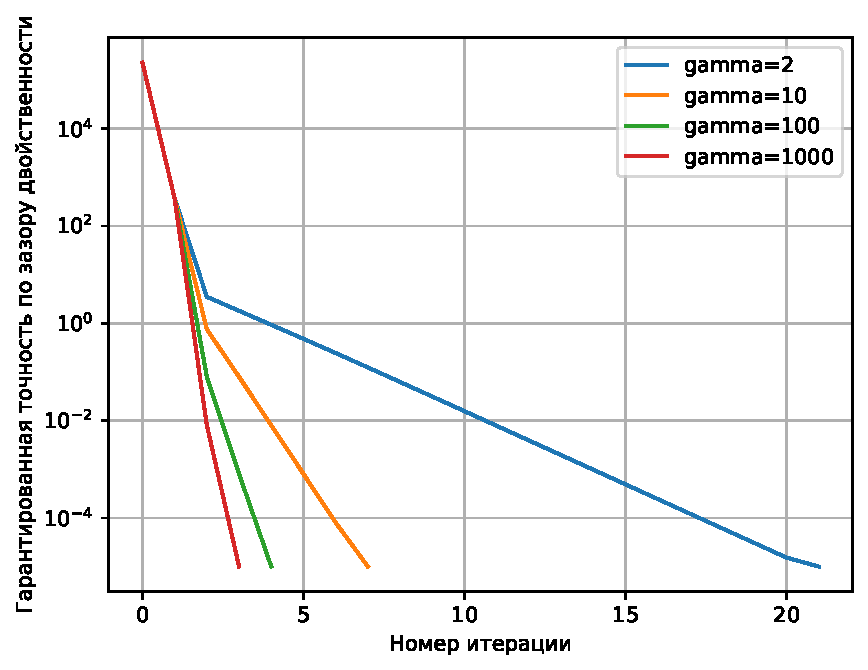
\includegraphics[width=.4\textwidth]{pics/1/barrier_lasso_gap_vs_iter_gamma_abalone.pdf}
 		} &

		\subfloat{
    		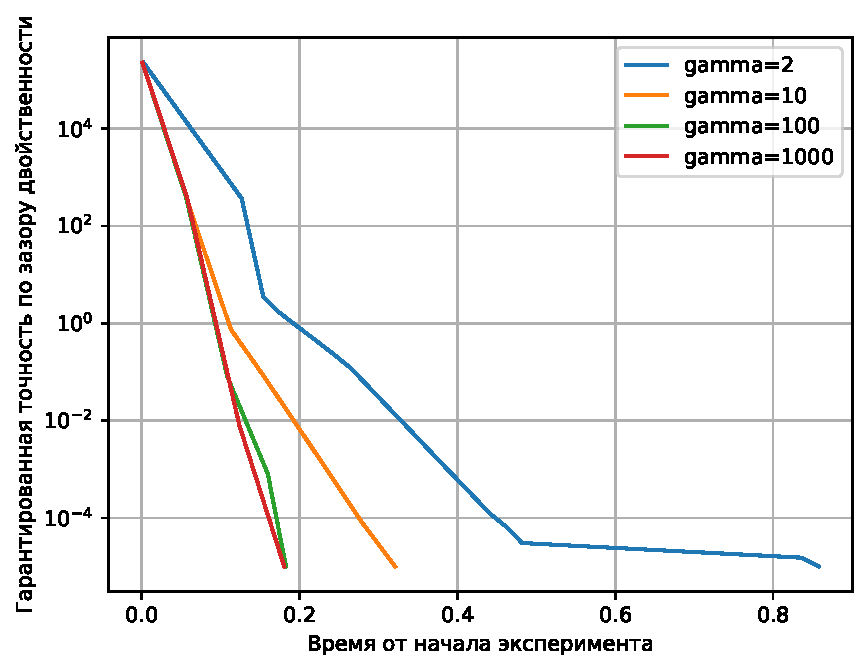
\includegraphics[width=.4\textwidth]{pics/1/barrier_lasso_gap_vs_time_gamma_abalone.pdf}
 		}
   \end{tabular}
   \captionsetup{justification=centering}
   \caption{Поведение метода логарифмических барьеров с разными значениями $\gamma$ на наборе данных abalone}
\end{figure}

\begin{figure}[H]
	\captionsetup{font=scriptsize}
	\centering
	\begin{tabular}[c]{cc}
		\subfloat{
    		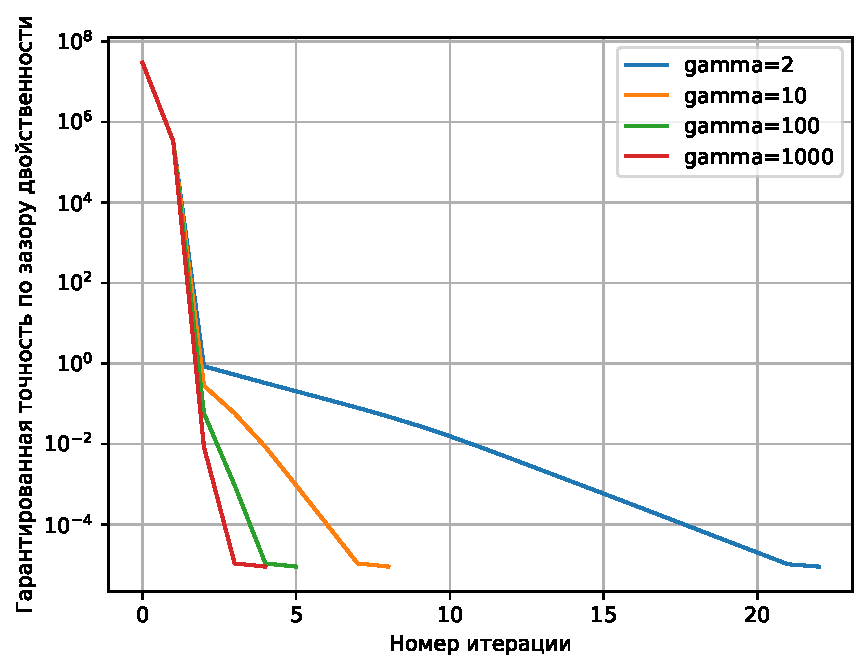
\includegraphics[width=.4\textwidth]{pics/1/barrier_lasso_gap_vs_iter_gamma_cpusmall.pdf}
 		} &

		\subfloat{
    		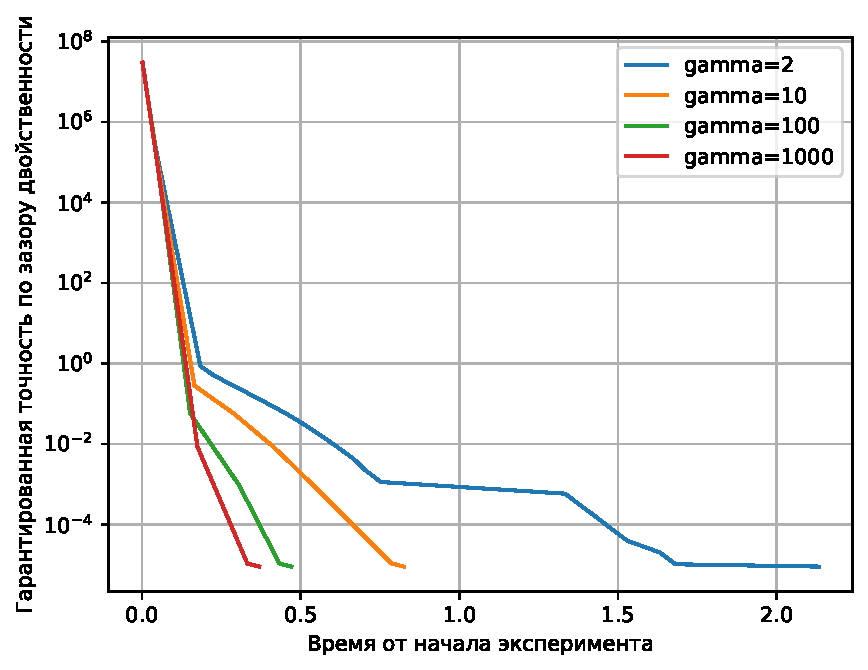
\includegraphics[width=.4\textwidth]{pics/1/barrier_lasso_gap_vs_time_gamma_cpusmall.pdf}
 		}
   \end{tabular}
   \captionsetup{justification=centering}
   \caption{Поведение метода логарифмических барьеров с разными значениями $\gamma$ на наборе данных cpusmall}
\end{figure}


\begin{figure}[H]
	\captionsetup{font=scriptsize}
	\centering
	\begin{tabular}[c]{cc}
		\subfloat{
    		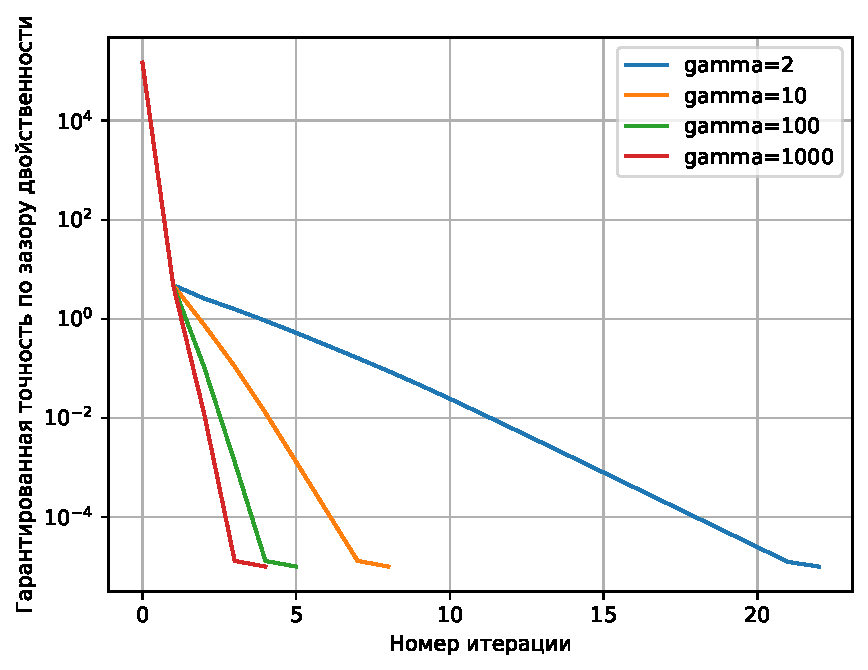
\includegraphics[width=.4\textwidth]{pics/1/barrier_lasso_gap_vs_iter_gamma_housing.pdf}
 		} &

		\subfloat{
    		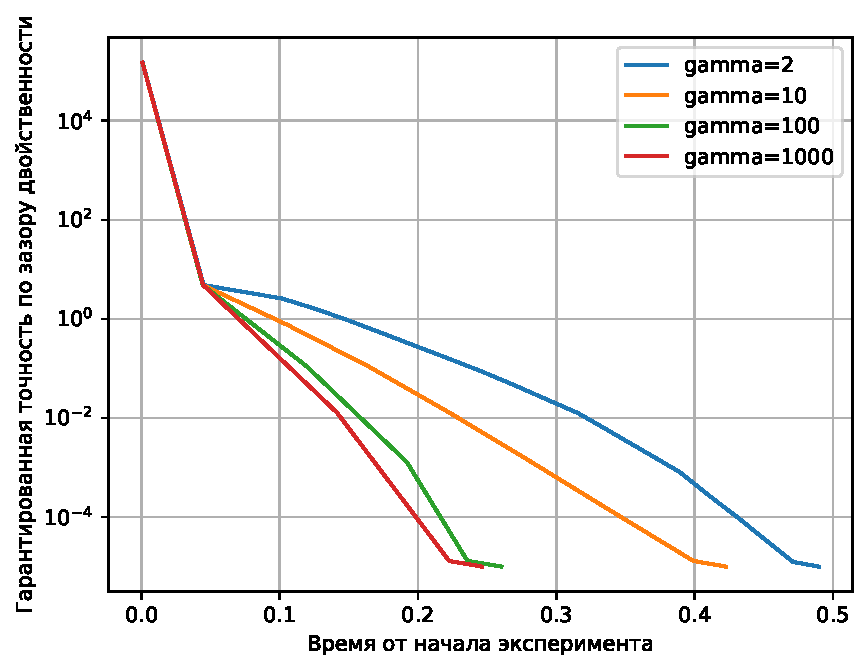
\includegraphics[width=.4\textwidth]{pics/1/barrier_lasso_gap_vs_time_gamma_housing.pdf}
 		}
   \end{tabular}
   \captionsetup{justification=centering}
   \caption{Поведение метода логарифмических барьеров с разными значениями $\gamma$ на наборе данных housing}
\end{figure}

\begin{figure}[H]
	\captionsetup{font=scriptsize}
	\centering
	\begin{tabular}[c]{cc}
		\subfloat{
    		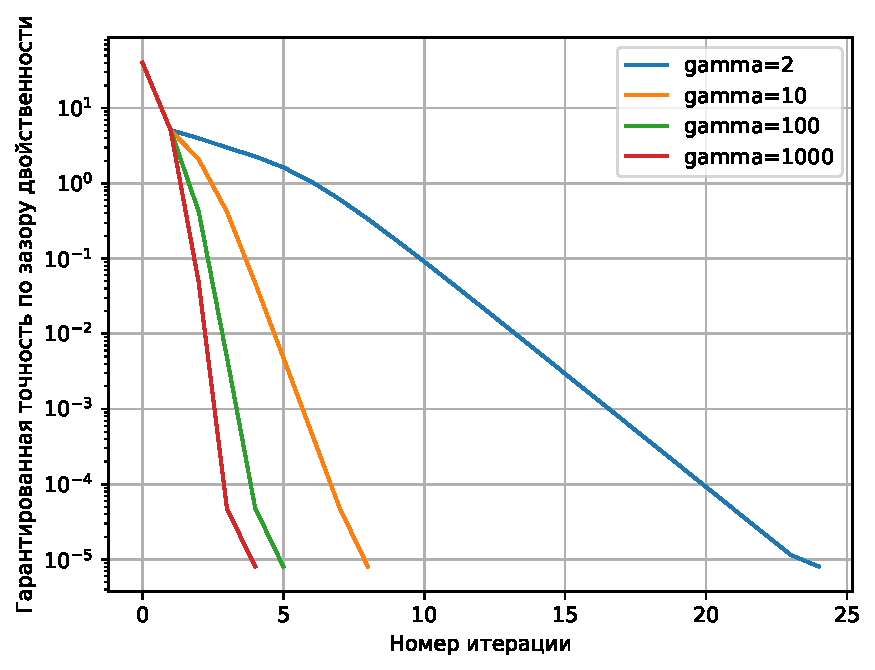
\includegraphics[width=.4\textwidth]{pics/1/barrier_lasso_gap_vs_iter_gamma_triazines.pdf}
 		} &

		\subfloat{
    		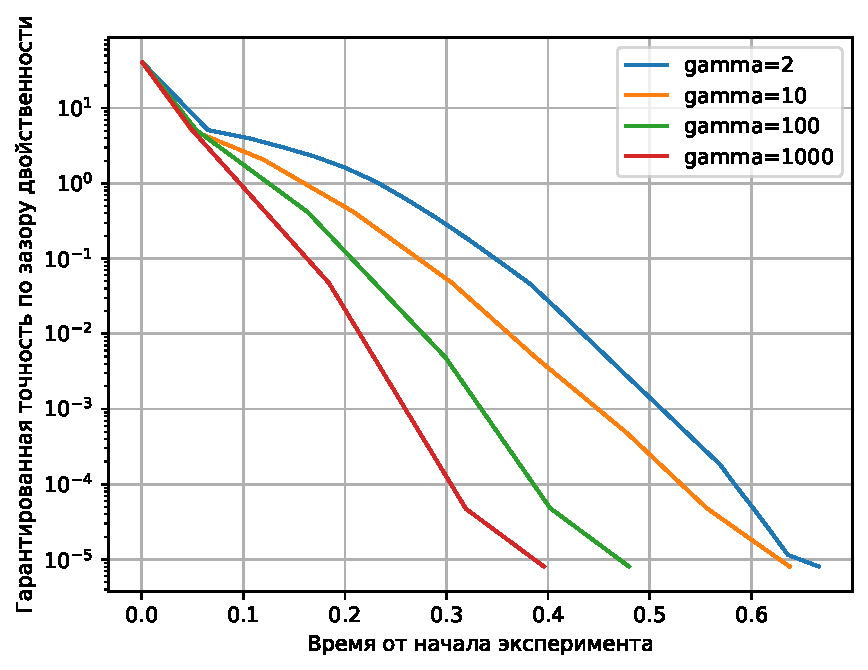
\includegraphics[width=.4\textwidth]{pics/1/barrier_lasso_gap_vs_time_gamma_triazines.pdf}
 		}
   \end{tabular}
   \captionsetup{justification=centering}
   \caption{Поведение метода логарифмических барьеров с разными значениями $\gamma$ на наборе данных triazines}
\end{figure}

\subsubsection{Зависимость поведения метода от $\varepsilon_{inner}$}

\begin{figure}[H]
	\captionsetup{font=scriptsize}
	\centering
	\begin{tabular}[c]{cc}
		\subfloat{
    		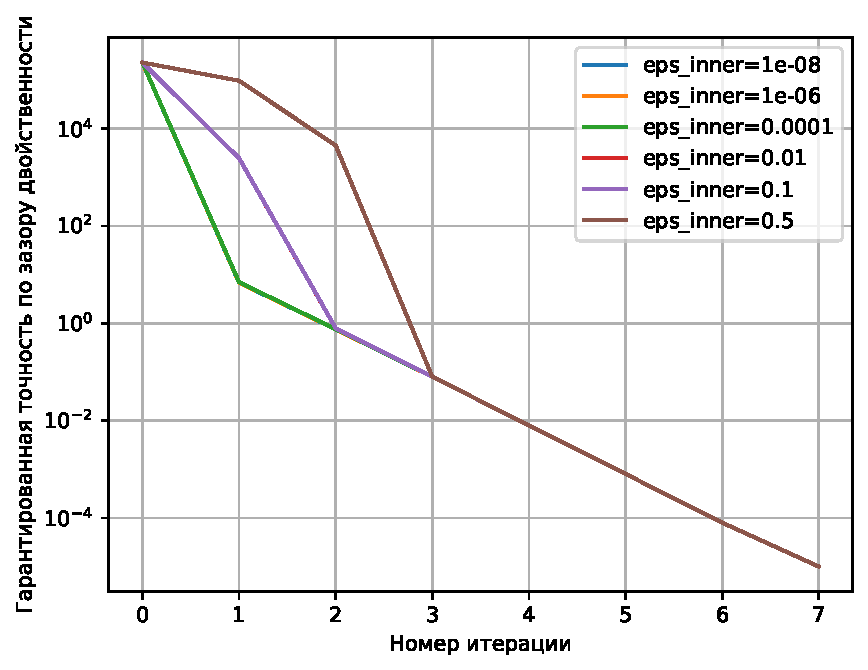
\includegraphics[width=.4\textwidth]{pics/1/barrier_lasso_gap_vs_iter_inner_eps_abalone.pdf}
 		} &

		\subfloat{
    		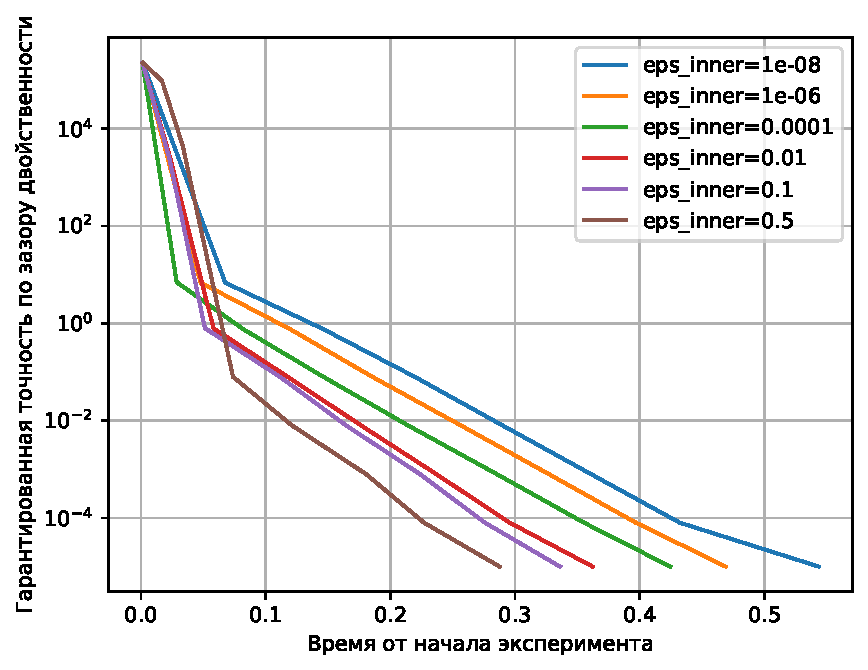
\includegraphics[width=.4\textwidth]{pics/1/barrier_lasso_gap_vs_time_inner_eps_abalone.pdf}
 		}
   \end{tabular}
   \captionsetup{justification=centering}
   \caption{Поведение метода логарифмических барьеров с разными значениями $\varepsilon_{inner}$ на наборе данных abalone}
\end{figure}

\begin{figure}[H]
	\captionsetup{font=scriptsize}
	\centering
	\begin{tabular}[c]{cc}
		\subfloat{
    		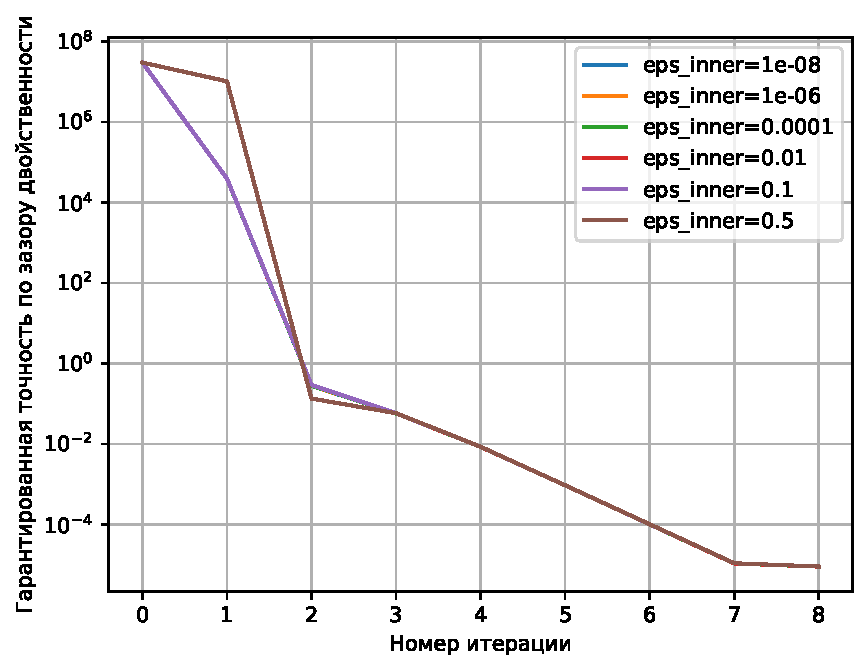
\includegraphics[width=.4\textwidth]{pics/1/barrier_lasso_gap_vs_iter_inner_eps_cpusmall.pdf}
 		} &

		\subfloat{
    		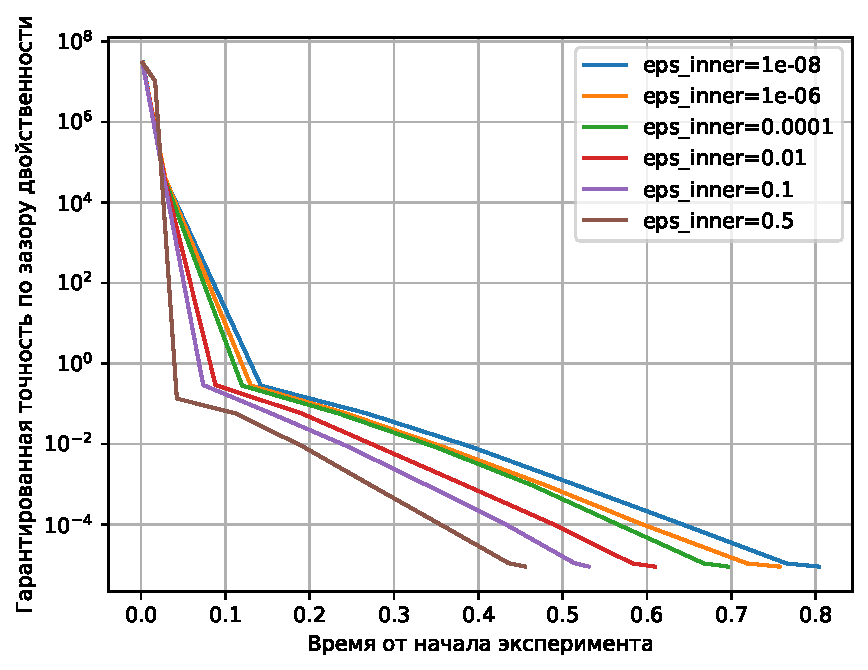
\includegraphics[width=.4\textwidth]{pics/1/barrier_lasso_gap_vs_time_inner_eps_cpusmall.pdf}
 		}
   \end{tabular}
   \captionsetup{justification=centering}
   \caption{Поведение метода логарифмических барьеров с разными значениями $\varepsilon_{inner}$ на наборе данных cpusmall}
\end{figure}


\begin{figure}[H]
	\captionsetup{font=scriptsize}
	\centering
	\begin{tabular}[c]{cc}
		\subfloat{
    		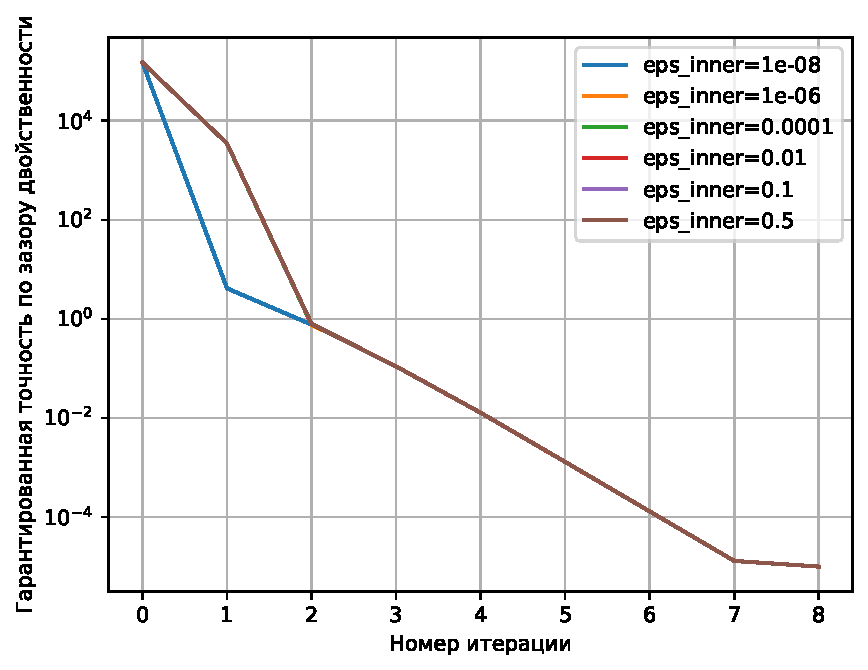
\includegraphics[width=.4\textwidth]{pics/1/barrier_lasso_gap_vs_iter_inner_eps_housing.pdf}
 		} &

		\subfloat{
    		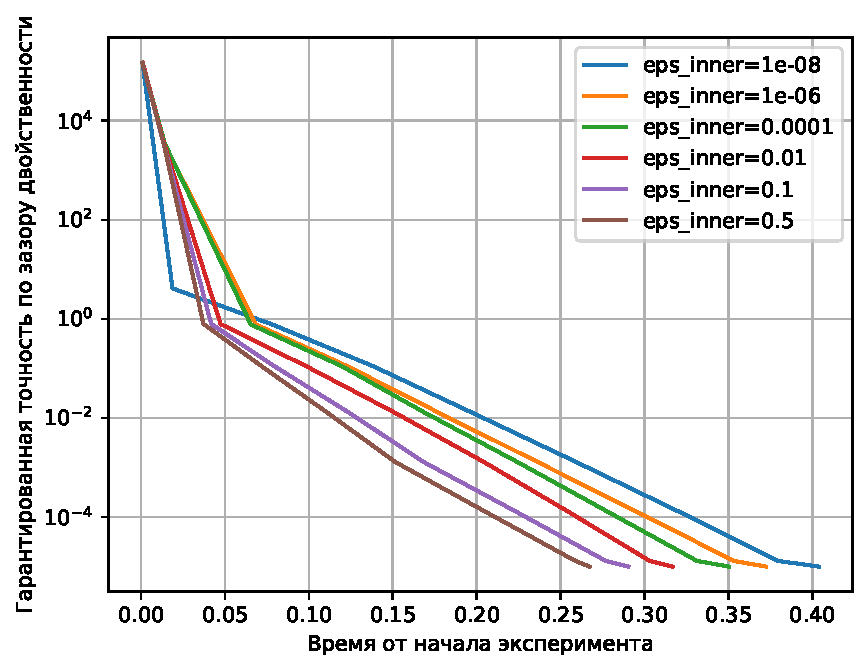
\includegraphics[width=.4\textwidth]{pics/1/barrier_lasso_gap_vs_time_inner_eps_housing.pdf}
 		}
   \end{tabular}
   \captionsetup{justification=centering}
   \caption{Поведение метода логарифмических барьеров с разными значениями $\varepsilon_{inner}$ на наборе данных housing}
\end{figure}

\begin{figure}[H]
	\captionsetup{font=scriptsize}
	\centering
	\begin{tabular}[c]{cc}
		\subfloat{
    		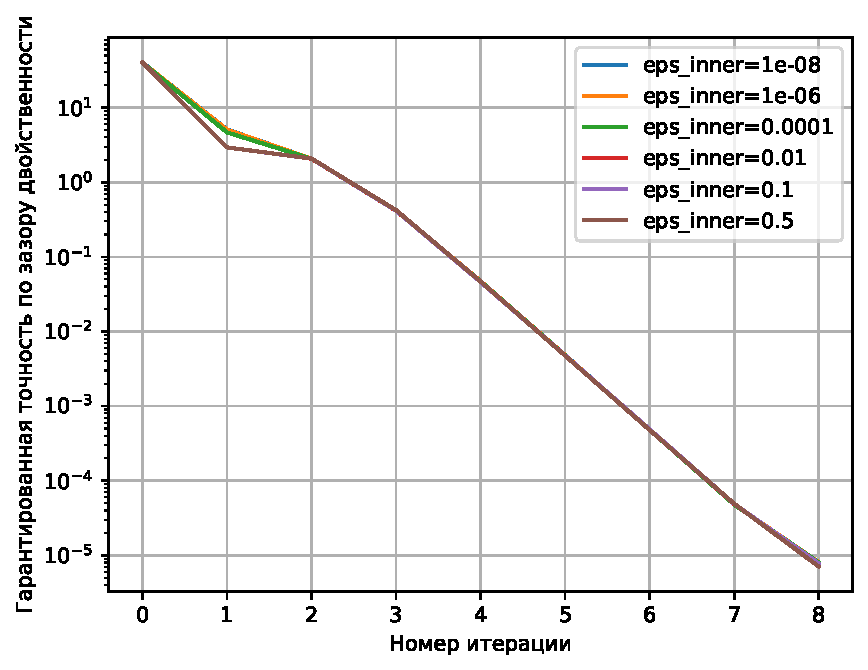
\includegraphics[width=.4\textwidth]{pics/1/barrier_lasso_gap_vs_iter_inner_eps_triazines.pdf}
 		} &

		\subfloat{
    		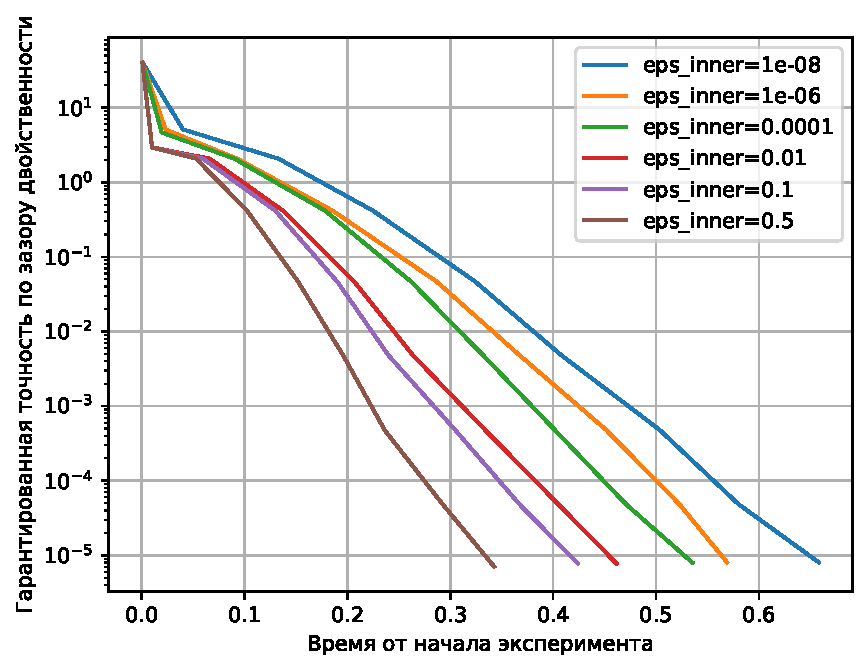
\includegraphics[width=.4\textwidth]{pics/1/barrier_lasso_gap_vs_time_inner_eps_triazines.pdf}
 		}
   \end{tabular}
   \captionsetup{justification=centering}
   \caption{Поведение метода логарифмических барьеров с разными значениями $\varepsilon_{inner}$ на наборе данных triazines}
\end{figure}

По графикам видно, что большие значения $\gamma$ дают более быструю сходимость. При разных значениях $\varepsilon_{inner}$ получается одно и то же число итераций, нужное для сходимости, но по времени выходит гораздо быстрее. Интересно, что даже низкие требования к точности метода Ньютона не наносят урона сходимости. Это легко объяснить: даже одна итерация метода Ньютона способна дать хороший прогресс в оптимизации, и, судя по всему, малую заданную точность внутренний метод достигает с большим запасом.

В целом, изменение этих параметров не слишком повлияло на работу алгоритма.

Алгоритм смог справиться с выборкой triazines, хотя всё же стоило бы сначала оставить в матрице только линейно независимые столбцы.

\subsection{Зависимость метода от размерности пространства $n$, размера выборки $m$ и коэффициентра регуляризации $\lambda$}

	Будем генерировать компоненты матрицы объектов-признаков и целевого вектора из стандартного нормального распределения.

За начальную точку возьмём $(x_0, u_0) = (0.1 * 1_n, 0.2 * 1_n)$.
Берем не $x_0 = 0$, так как в этом случае при больших значениях $\lambda$ (например, 100) метод будет сходиться за одну итерацию -- это не илллюстрирует общую зависимость.

\begin{figure}[H]
	\captionsetup{font=scriptsize}
	\centering
	\begin{tabular}[c]{cc}
		\subfloat{
    		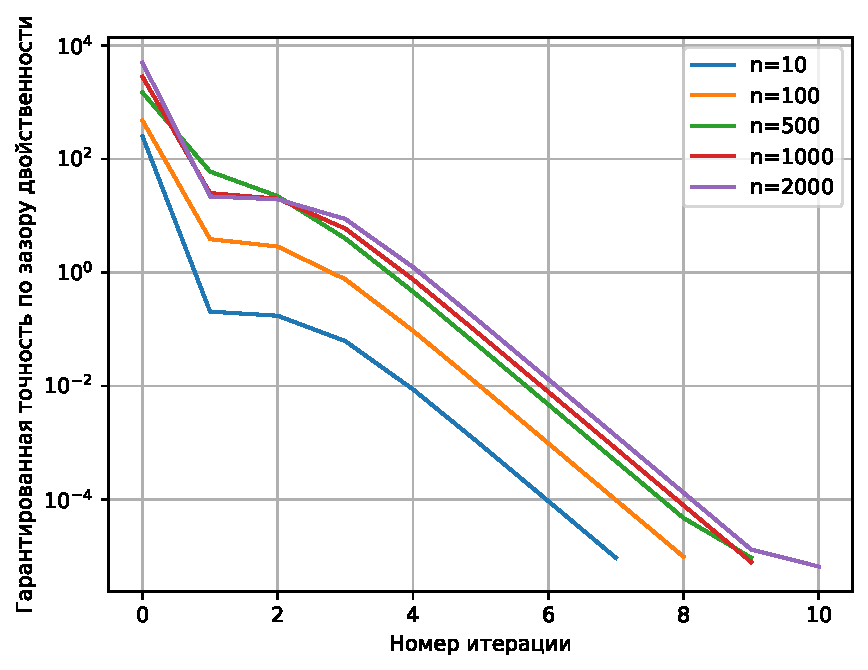
\includegraphics[width=.4\textwidth]{pics/2/barrier_lasso_gap_vs_iter_n.pdf}
 		} &

		\subfloat{
    		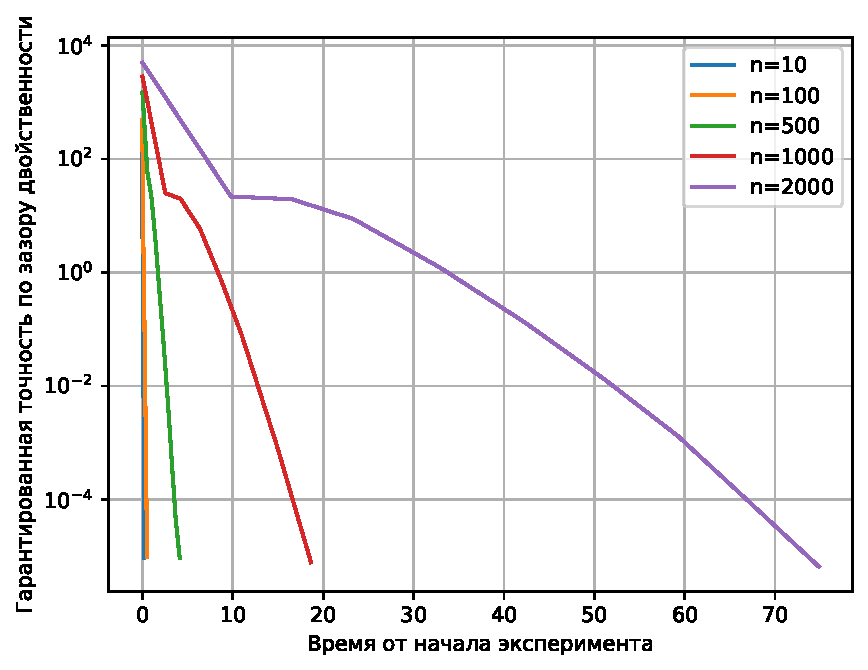
\includegraphics[width=.4\textwidth]{pics/2/barrier_lasso_gap_vs_time_n.pdf}
 		}
   \end{tabular}
   \captionsetup{justification=centering}
   \caption{Поведение метода логарифмических барьеров с разными значениями $n$}
\end{figure}

\begin{figure}[H]
	\captionsetup{font=scriptsize}
	\centering
	\begin{tabular}[c]{cc}
		\subfloat{
    		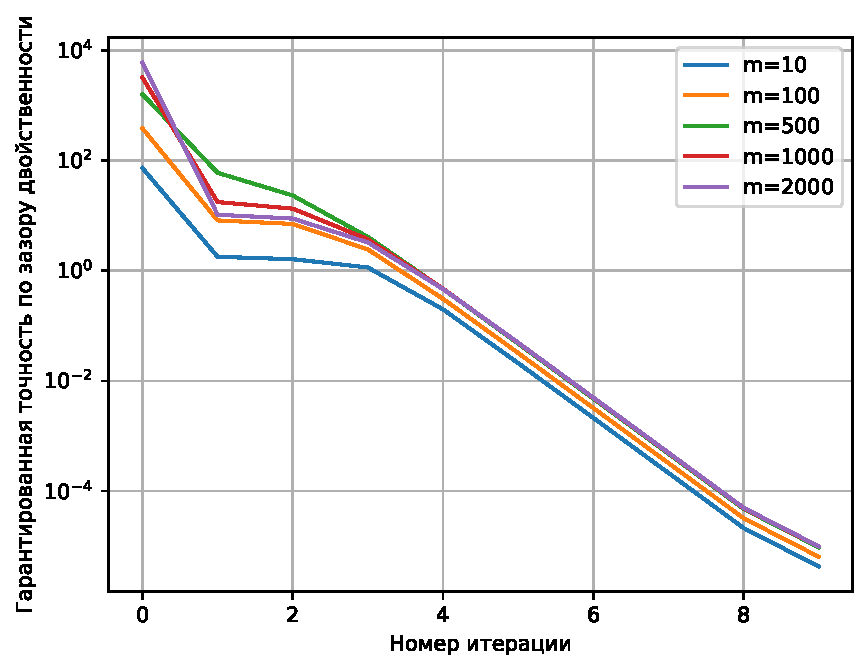
\includegraphics[width=.4\textwidth]{pics/2/barrier_lasso_gap_vs_iter_m.pdf}
 		} &

		\subfloat{
    		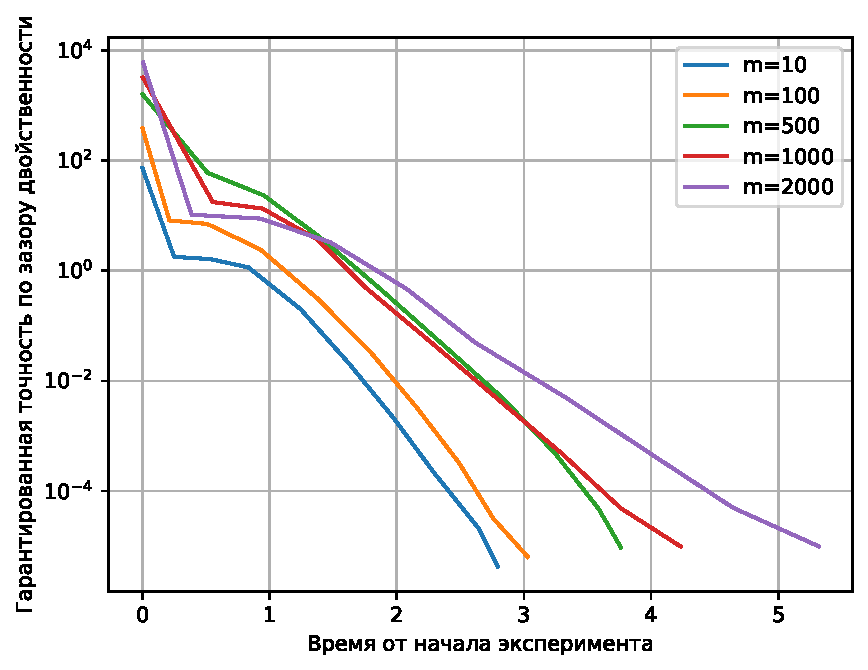
\includegraphics[width=.4\textwidth]{pics/2/barrier_lasso_gap_vs_time_m.pdf}
 		}
   \end{tabular}
   \captionsetup{justification=centering}
   \caption{Поведение метода логарифмических барьеров с разными значениями $m$}
\end{figure}

\begin{figure}[H]
	\captionsetup{font=scriptsize}
	\centering
	\begin{tabular}[c]{cc}
		\subfloat{
    		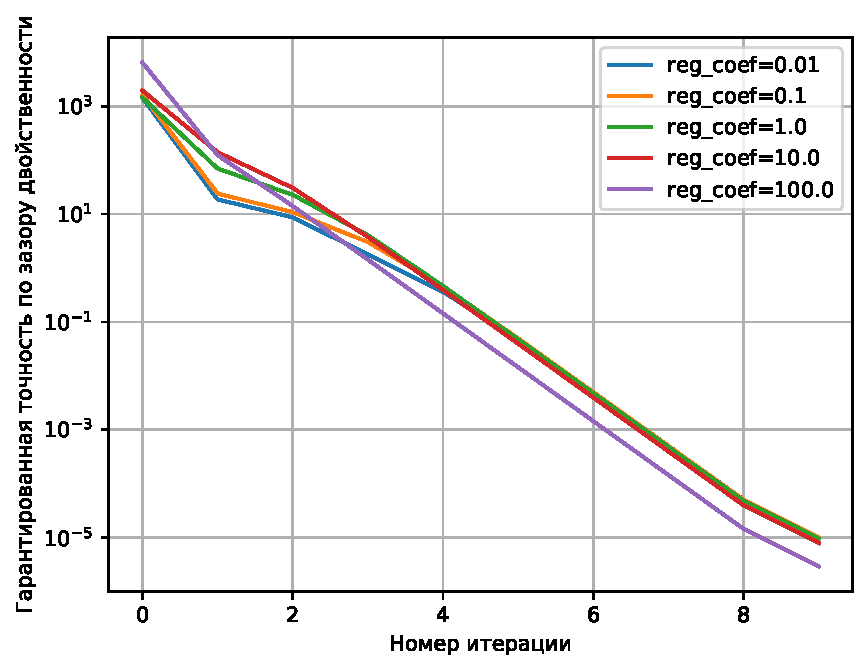
\includegraphics[width=.4\textwidth]{pics/2/barrier_lasso_gap_vs_iter_reg_coef.pdf}
 		} &

		\subfloat{
    		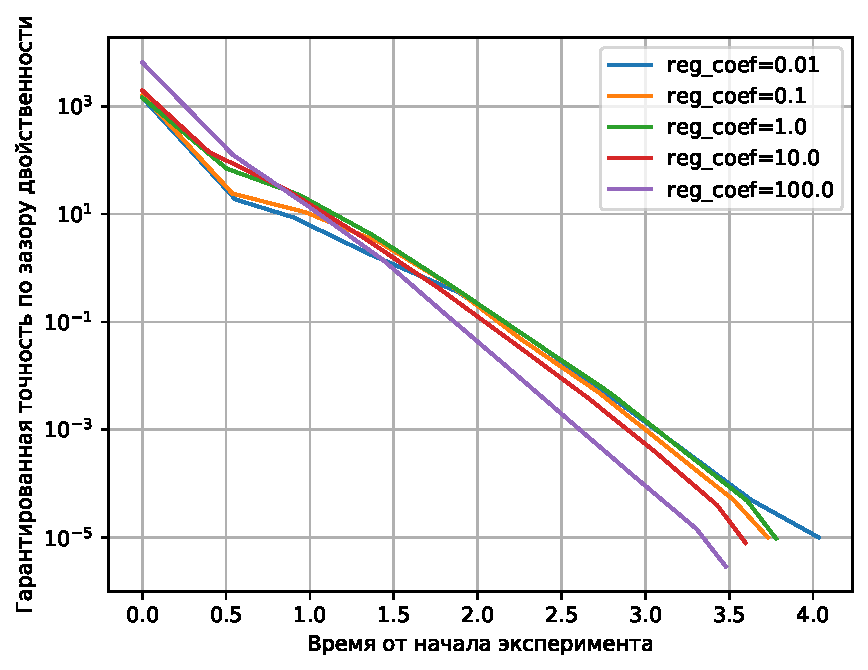
\includegraphics[width=.4\textwidth]{pics/2/barrier_lasso_gap_vs_time_reg_coef.pdf}
 		}
   \end{tabular}
   \captionsetup{justification=centering}
   \caption{Поведение метода логарифмических барьеров с разными значениями $\lambda$}
\end{figure}

Для меньших размерностей задача решается на пару итераций быстрее, при этом требуемое время существенно вырастает с ростом $n$, что очевидным образом объясняется кубической от $n$ стоимостью итерации метода Ньютона. 

С изменением $m$ число требуемых итераций изменяется ещё меньше.
Требуемое время растёт -- линейная зависимость стоимости итерации метода Ньютона от $m$.

Число внешних итераций не меняется при изменении $\lambda$, но они требуют меньше времени, что можно объяснить тем, что решение становится проще с ростом $\lambda$, и при $\lambda \geq\left\|A^{T} b\right\|_{\infty}$  $x_{opt} = 0$.

\section{Выводы.}
Мы изучили метод логарифмических барьеров для решения задач условной оптимизации на примере LASSO-регрессии. Было показано влияние гиперпараметров метода на его работу.
\end{document}